%%%%%%%%%%%%%%%%%%%%%%%%%%%%%%%%%%%%%%%%%
% Beamer Presentation
% LaTeX Template
% Version 1.0 (10/11/12)
%
% This template has been downloaded from:
% http://www.LaTeXTemplates.com
%
% License:
% CC BY-NC-SA 3.0 (http://creativecommons.org/licenses/by-nc-sa/3.0/)
%
%%%%%%%%%%%%%%%%%%%%%%%%%%%%%%%%%%%%%%%%%

%----------------------------------------------------------------------------------------
%	PACKAGES AND THEMES
%----------------------------------------------------------------------------------------

\documentclass{beamer}

\mode<presentation> {

% The Beamer class comes with a number of default slide themes
% which change the colors and layouts of slides. Below this is a list
% of all the themes, uncomment each in turn to see what they look like.

%\usetheme{default}
%\usetheme{AnnArbor}
%\usetheme{Antibes}
%\usetheme{Bergen}
%\usetheme{Berkeley}
%\usetheme{Berlin}
%\usetheme{Boadilla}
%\usetheme{CambridgeUS}
%\usetheme{Copenhagen}
%\usetheme{Darmstadt}
%\usetheme{Dresden}
%\usetheme{Frankfurt}
%\usetheme{Goettingen}
%\usetheme{Hannover}
%\usetheme{Ilmenau}
%\usetheme{JuanLesPins}
%\usetheme{Luebeck}
\usetheme{Madrid}
%\usetheme{Malmoe}
%\usetheme{Marburg}
%\usetheme{Montpellier}
%\usetheme{PaloAlto}
%\usetheme{Pittsburgh}
%\usetheme{Rochester}
%\usetheme{Singapore}
%\usetheme{Szeged}
%\usetheme{Warsaw}

% As well as themes, the Beamer class has a number of color themes
% for any slide theme. Uncomment each of these in turn to see how it
% changes the colors of your current slide theme.

%\usecolortheme{albatross}
%\usecolortheme{beaver}
%\usecolortheme{beetle}
%\usecolortheme{crane}
%\usecolortheme{dolphin}
%\usecolortheme{dove}
%\usecolortheme{fly}
%\usecolortheme{lily}
%\usecolortheme{orchid}
%\usecolortheme{rose}
%\usecolortheme{seagull}
%\usecolortheme{seahorse}
%\usecolortheme{whale}
%\usecolortheme{wolverine}

%\setbeamertemplate{footline} % To remove the footer line in all slides uncomment this line
%\setbeamertemplate{footline}[page number] % To replace the footer line in all slides with a simple slide count uncomment this line

%\setbeamertemplate{navigation symbols}{} % To remove the navigation symbols from the bottom of all slides uncomment this line
}

\usepackage{graphicx} % Allows including images
\usepackage{bm}
\usepackage{booktabs} % Allows the use of \toprule, \midrule and \bottomrule in tables
\usepackage{color}
\usepackage{tikz}
\usepackage{amsmath}
\usepackage{framed}

\usetikzlibrary{topaths,calc}

\AtBeginSection[]{
  \begin{frame}
  \vfill
  \centering
  \begin{beamercolorbox}[sep=8pt,center,shadow=true,rounded=true]{title}
    \usebeamerfont{title}\insertsectionhead\par%
  \end{beamercolorbox}
  \vfill
  \end{frame}
}
%----------------------------------------------------------------------------------------
%	TITLE PAGE
%----------------------------------------------------------------------------------------
\title[Short title]{Knowledge Compilation und \#SAT}

\author{Narek Bojikian} % Your name
\institute[Hu-Berlin] % Your institution as it will appear on the bottom of every slide, may be shorthand to save space
{
Humboldt University of Berlin\\ % Your institution for the title page
}
\date{08.01.2019} % Date, can be changed to a custom date

\begin{document}

\begin{frame}
\titlepage % Print the title page as the first slide
\end{frame}

\begin{frame}[t]{Definitions}
\begin{itemize}
\uncover<1->{\item The SAT Problem (\textbf{SAT}).}
\uncover<2->{\item Counting SAT Problem (\textbf{\#SAT}).}


\uncover<6->{\item Negation Normal Form (\textbf{NNF}).}
\uncover<7->{\item Conjunctive Normal Form (\textbf{CNF}).}
\uncover<8->{\item Decomposable Negation Normal Form (\textbf{DNNF}).}
\uncover<9->{\item deterministic Decomposable Negation Normal Form (\textbf{d-DNNF}).}
\uncover<10->{\item decision Decomposable Negation Normal Form (\textbf{dec-DNNF}).}
\end{itemize}

\only<1>{
\begin{block}{SAT}
\begin{itemize}
\item[--] Given a Boolean formula $\phi$ of $n$ variables.
\item[?] Find an assignment that satisfies $\phi$.
\end{itemize}
\end{block}
}

\only<2>{
\begin{block}{\#SAT}
\begin{itemize}
\item[--] Given a Boolean formula $\phi$ of $n$ variables.
\item[?] How many assignments in $2^{\mathrm{Var}(\phi)}$ satisfy $\phi$?
\end{itemize}
\end{block}
}

\only<3-4>{
\begin{block}{Notation}
Let $\mathrm{SAT}(\chi) \subseteq 2^{\mathrm{VAR}(\chi)}$ be the set of all satisfying assignments of $\chi$
\vspace{-0.3cm}
$$\mathrm{SAT}(\chi) = \{\rho:\mathrm{VAR}(\chi) \rightarrow \{0, 1\} : \rho(\chi) = 1\}.$$
\vspace{-0.8cm}
\uncover<4->{$$\text{SAT: Is } \mathrm{SAT}(\phi) = \emptyset.
\qquad \qquad \qquad
\text{\#SAT: Find } |\mathrm{SAT}(\phi)|.$$}
\vspace{-0.6cm}
\end{block}
}

\only<5>{
\begin{block}{Example}
$$\phi = X_1 \land (X_2 \lor \lnot X_3)$$
Clearly, \#SAT($\phi$) = 3.
\end{block}
}

\only<6>{
\begin{block}{Negation Normal Form}
A Boolean formula $\phi$ is in NNF form, if it contains only disjunctions and conjunctions over a set of positive and(or) negative literals.

\textbf{Example.} $\phi = X_1 \lor \lnot X_2$.
\end{block}
}

\only<7>{
\begin{block}{Conjunctive Normal Form}
A Boolean formula $\phi$ is in CNF, if it is a conjunction of one or more clauses, where each clauses is a disjunction of one or more literals. Note that each CNF formula is an NNF formula as well.
\end{block}
}

\only<8>{
\begin{block}{Decomposable Negation Normal Form}
A Boolean formula $\phi$ is in DNNF, if it is in NNF and for each conjunction subformula $phi' := \psi_1 \land \psi_2$ we have $\mathrm{VAR}(\psi_1) \cap \mathrm{VAR}(\psi_2) = \emptyset$.
\end{block}
}

\only<9>{
\begin{block}{deterministic Decomposable Negation Normal Form}
A Boolean formula $\phi$ is in d-DNNF, if it is in DNNF and for each disjunction subformula  $\phi' = \psi_1 \lor \psi_2$ we have $\mathrm{SAT}(\psi_1) \cap \mathrm{SAT}(\psi_2) = \emptyset$.
\end{block}
}

\only<10->{
\begin{block}{decision Decomposable Negation Normal Form}
A Boolean formula $\phi$ is in dec-DNNF, if it is in DNNF and each disjunction subformula  $\phi'$ is of the form $\phi' = (X \land \psi_1) \lor (\lnot X \land \psi_2)$ for some variable $X \in \mathrm{VAR}(\phi)$.

\uncover<11>{\textbf{Note.} Each dec-DNNF is a d-DNNF.}
\end{block}
}
\end{frame}

\begin{frame}[t]{Structuredness of a formula}
	\begin{itemize}[<+->]
		\item Let $\phi$ be a DNNF formula and let $V := \mathrm{VAR}(\phi)$.
		\item A \textbf{$\mathbf{v}$Tree} $T$ is a binary tree where the leaves of the tree has a one-to-one correspondence to the variables of $\phi$.
		\item The formula $\phi$ respects $T$ if and only if for each subformula of  $\phi$ of the form $\phi' := \psi_1 \land \psi_2$, there is a vertex $v \in V(T)$ with two children $v_1, v_2$, where $\mathrm{VAR}(\psi_1)\subseteq V(T_{v_1})$ and $\mathrm{VAR}(\psi_2) \subseteq V(T_{v_2})$, where $T_v$ is the subtree of $T$ rooted at $v$. We say $\phi'$ respects $v$ in this case.
		\item A formula $\phi$ is structured, if there is a $v$tree $T$ over the vertices of $\phi$, such that $\phi$ respects $T$.
	\end{itemize}

	\uncover<3->{
	\begin{minipage}{.49\linewidth}
		$$(x\land(y\lor z)) \lor (z \textcolor{red}{\bm{\land}} \lnot x)$$
	\end{minipage}
	\hfill
	\begin{minipage}{.49\linewidth}
		\centering
		\includegraphics[width=.6\linewidth]{figures/vtree.eps}
	\end{minipage}
	}
\end{frame}

\begin{frame}[t]{Hypergraphs and $\beta$-acyclic graphs}
	\begin{minipage}{.59\linewidth}
	\begin{itemize}
		\item Hypergraphs $\mathcal{G}$.
			\begin{itemize}
				\item A set of vertices $V(\mathcal{G})$.
				\item Edges $E(\mathcal{G})$, defined as 
				\item[] subsets over $V(\mathcal{G})$.
			\end{itemize}
		\item Different ways to translate
		\item[] \hspace{1cm} to hypergraphs.
		\item $\beta$ acyaclic hypergraphs.
			\begin{itemize}
				\item Defined on the edges.
				\item Let $\rho := v_1, \dots v_n$ be an
				\item[] \hspace{1cm}enumeration of the vertices.
				\item $\rho$ is an $\beta$-elimination, if for all
				\item[] \hspace{1cm}$e_1, e_2 \in E(\mathcal{G})$ and $v_i \in e_1 \cap e_2$,
				\item[]\hspace{1cm}$e_{1|\geq i} \subseteq e_2$ or $e_{2|\geq i} \subseteq e_1$.
				\item A hypergraph is $\beta$-acyclic,
				\item[] \hspace{1cm} if it admits an elimination.

			\end{itemize}
	\end{itemize}
\end{minipage}
\begin{minipage}{.39\linewidth}
\centering
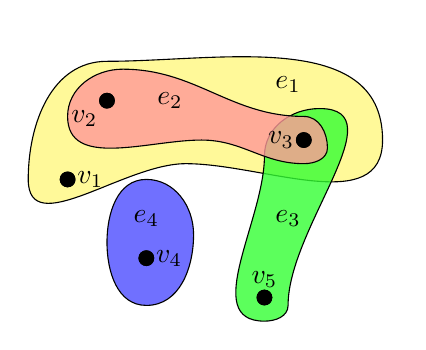
\begin{tikzpicture}
    \node (v1) at (1,2) {};
    \node (v2) at (1.5,3) {};
    \node (v3) at (4,2.5) {};
    \node (v4) at (2,1) {};
    \node (v5) at (3.5,0.5) {};

    \begin{scope}[fill opacity=0.8]
    \filldraw[fill=yellow!50] ($(v1)+(-0.5,0)$) 
        to[out=90,in=180] ($(v2) + (0,0.5)$) 
        to[out=0,in=90] ($(v3) + (1,0)$)
        to[out=270,in=0] ($(v2) + (1,-0.8)$)
        to[out=180,in=270] ($(v1)+(-0.5,0)$);
    \filldraw[fill=blue!70] ($(v4)+(-0.5,0.2)$)
        to[out=90,in=180] ($(v4)+(0,1)$)
        to[out=0,in=90] ($(v4)+(0.6,0.3)$)
        to[out=270,in=0] ($(v4)+(0,-0.6)$)
        to[out=180,in=270] ($(v4)+(-0.5,0.2)$);

    \filldraw[fill=green!80] ($(v3)+(-0.5,-0.2)$) 
        to[out=90,in=180] ($(v3) + (0.2,0.4)$) 
        to[out=0,in=90] ($(v5) + (0.3,-0.1)$)
        to[out=270,in=0] ($(v5) + (0,-0.3)$)
        to[out=180,in=270] ($(v3)+(-0.5,-0.2)$);

    \filldraw[fill=red!40] ($(v2)+(-0.5,-0.2)$) 
        to[out=90,in=180] ($(v2) + (0.2,0.4)$) 
        to[out=0,in=180] ($(v3) + (0,0.3)$)
        to[out=0,in=90] ($(v3) + (0.3,-0.1)$)
        to[out=270,in=0] ($(v3) + (0,-0.3)$)
        to[out=180,in=0] ($(v3) + (-1.3,0)$)
        to[out=180,in=270] ($(v2)+(-0.5,-0.2)$);
    \end{scope}

    \foreach \v in {1,2,...,5} {
        \fill (v\v) circle (0.1);
    }

    \fill (v1) circle (0.1) node [right] {$v_1$};
    \fill (v2) circle (0.1) node [below left] {$v_2$};
    \fill (v3) circle (0.1) node [left] {$v_3$};
    \fill (v4) circle (0.1) node [right] {$v_4$};
    \fill (v5) circle (0.1) node [above] {$v_5$};

    \node at (3.8,3.2) {$e_1$};
    \node at (2.3,3) {$e_2$};
    \node at (3.8,1.5) {$e_3$};
    \node at (2, 1.5) {$e_4$};
\end{tikzpicture}

\end{minipage}
\footnotetext[1]{$e_{|\geq i} := e \cap \{v_i, \dots v_n\}$.}
\end{frame}

\begin{frame}[t]{Incidence graphs and structure of formulas}
	\begin{itemize}
		\item The \textbf{incidence graph} of $\mathcal{G}$ is a 
		\item[] \hspace{1cm}bipartite graph $(V(\mathcal{G}) \cup E(\mathcal{G}), E)$
		\item[] \hspace{1cm},where $\{v, e\} \in E$ iff $v \in e$.
			\vspace{.5cm}
		\item Hypergraph of a CNF-Formula.
		\item The incidence graph of a CNF-Formula is 
		\item[] \hspace {1cm} the incidence graph of its hyper graph.
		\item A CNF-Formula is $\beta$-acyclic if its hypergraph is.
	\end{itemize}

\end{frame}
	


\section{Polynomial upper-bound on the practical method}
\begin{frame}[t]{Lemmas on $\beta$-acyclic graphs}
	\begin{itemize}
		\item We fix a $\beta$-acyclic graph $\mathcal{H}$ and an elimination-ordering $\leq$ on $\mathcal{H}$.
		\item Let $v_1, \dots v_n$ be an enumeration of the vertices in $\mathcal{H}$ according to $\leq$.
		\item $V_{\leq v_i} := \{v_j ; j\leq i\}$.
		\item For two edge $e, f \in \mathcal{H}$, $e < f$ if and only if $\max\{e \Delta f\}\in f$
	\end{itemize}
	\begin{block}{Lemma (lemma 2)}
		For $x,y \in V(\mathcal{H}), x \leq y$ and for $e, f \in \mathcal{H}, e \leq f$,
			$$\text{if } V(\mathcal{H}^x_e)\cap V(\mathcal{H}^y_f)\cap V_{\leq x} \neq \emptyset,
			\text{ then } \mathcal{H}^x_e \subseteq \mathcal{H}^y_f.$$
		In particular, for all $y$,
		$$\text{if } e \in \mathcal{H}^y_f, \text{ then } \mathcal{H}^y_e \subseteq \mathcal{H}^y_f$$
	\end{block}
\end{frame}

\begin{frame}[t]{Lemmas on $\beta$-acyclic graphs}
	\begin{block}{Lemma (lemma 4)}
		For $e, f \in \mathcal{H}, e\leq f$, If there exists a vertex $x \in V(\mathcal{H})$, such that $x \in e \cap f$, then $e \cap V_{\geq x} \subseteq f$.
	\end{block}
\end{frame}

\begin{frame}[t]{Lemmas on $\beta$-acyclic graphs}
	A decreasing path from $e$ to $f$ is a path $(e_0, x_0, e_1, v_1 \dots v_{l-1}, e_n)$, such that 
	\begin{block}{Lemma (lemma 5)}
		For $x \in V(\mathcal{H}), e \in \mathcal{H}$ and $f \in \mathcal{H}^x_e$, there exists a decreasing path from $e$ to $f$ going through vertices smaller than $x$.
	\end{block}
	Proof sketch. Any shortest path from $e$ to $f$ is decreasing. A path exists by definition [see below].

\end{frame}

\begin{frame}[t]{Lemmas on $\beta$-acyclic graphs}
	\begin{block}{Theorem (theorem 3)}
		For every $x \in V(\mathcal{H})$ and $e \in \mathcal{H}, V(\mathcal{H}^x_e) \cap V_{\geq x} \subseteq e$
	\end{block}

	[figure]

	[why do we need this]
\end{frame}


\begin{frame}[t]{Solving \#SAT in $\beta$-acyclic graphs}
	\begin{itemize}
		\item For a clause $C$, we define the partial assignment $\tau_C$ over the variables of $C$ as the only assignment that does not satisfies $C$, i.e. for $x \in C$, $\tau_C(x) = 1$ if and only if $x$ appears as a negative literal in $C$.

		\item Let $F$ be a given $\beta$-acyclic CNF-formula and $v_1, \dots v_n$ be an elimination order of the variables in $F$. Let $\mathcal{H}$ be the hypergraph of $F$.
	\end{itemize}
	\begin{block}{Lemma (lemma 6)}
		Let $x \neq x_1 \in \mathrm{VAR}(F)$ and let $y$ be the predecessor of $x$ for $<$.  Let $e \in \mathcal{H}$ and $\tau : (e \cap V_{\geq x}) \rightarrow \{0, 1\}$. Then either $F^x_e[\tau] \equiv 1$ or there exists $U \subseteq \mathcal{H}^x_e$ such that 
		$$ F^x_e[\tau] \equiv \bigwedge\limits_{g \in U} F^y_g[\tau^y_{C_g}],$$
		where $C_g in F^x_e$ such that $\mathrm{C_g} = g$.
	\end{block}
\end{frame}

\begin{frame}[t]{Solving \#SAT in $\beta$-acyclic graphs}
		$$ F^x_e[\tau] \equiv \bigwedge\limits_{g \in U} F^y_g[\tau^y_{C_g}]$$
\end{frame}

\begin{frame}[t]{Solving \#SAT in $\beta$-acyclic graphs}
	\begin{block}{Corollary (corollary 7)}
		Let $x \neq x_1 \in \mathrm{VAR}(F)$ and let $y$ be the predecessor of $x$ for $<$. For every $C \in \mathcal{H}$, there exist $U_0, U_1 \subseteq \mathcal{H}^x_{\mathrm{VAR}(C)}$ such that
		$$F^x_{\mathrm{VAR}(C)}[\tau^x_C] \equiv 
		( x \land \bigwedge\limits_{g \in U_1} F^y_g[\tau^y_{C_g}]) \lor
		( \lnot x \land \bigwedge\limits_{g \in U_2} F^y_g[\tau^y_{C_g}])
		$$
	\end{block}
	Explanation.
\end{frame}

\begin{frame}[t]{Solving \#SAT in $\beta$-acyclic graphs}
	\begin{block}{Theorem (theorem 8)}
		Let $F$ be a $\beta$-acyclic CNF-formula. One can construct in polynomial time in $\mathrm{size}(F)$ a dec-DNNF $D$ of size $O(\mathrm(size(F))$ and fanin at most $|\mathcal{H}|$ computing F.
	\end{block}
\end{frame}

\section{Lower-bound on the theoretical method}
\begin{frame}[t]{Branch decomposition and MIM-width}
	\begin{itemize}[<+->]
		\item A \textbf{branch decomposition} $T$ of a graph $G = (V, E)$ is a binary rooted tree $T$, whose leaves are in one-to-one correspondence with $V$.
		\item The maximal-induced-matching width (MIM-width) of a vertex $t$ of $T$ is the size of a largest induced matching $M$ of $G[V\setminus V_t, V_t]$.
		\item $mimw(T) = \max\{\mathrm{mimw}(t) : t \in V(T)\}$.
	\end{itemize}

	\uncover<4->{
	Example.

	\begin{center}
		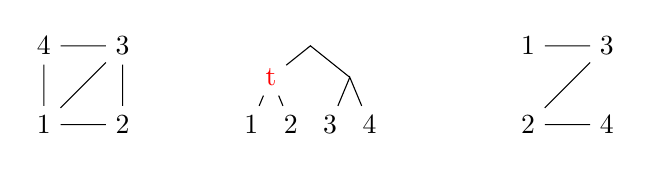
\begin{tikzpicture}
			\node (v1) at (0, 0){1};
			\node (v2) at (1, 0){2};
			\node (v3) at (1, 1){3};
			\node (v4) at (0, 1){4};
		
			\draw (v3) -- (v1) -- (v2) -- (v3) -- (v4) -- (v1);
		
		\begin{scope}[xshift = 75]
			\node (t1) at (0, 0){1};
			\node (t2) at (.5, 0){2};
			\node (t3) at (1, 0){3};
			\node (t4) at (1.5, 0){4};
			\node (t5) at (.25, .6){\color{red}t};
			\node (t6) at (1.25,.6){};
			\node (t7) at (.75, 1){};
			\draw (t1) -- (t5) -- (t2) (t3) -- (1.25, .6) -- (t4) (t5) to (.75, 1) to (1.25, .6);
		
		
		\end{scope}
		\begin{scope}[xshift = 175]
			\node (x1) at (0, 1){1};
			\node (x2) at (0, 0){2};
			\node (x3) at (1, 1){3};
			\node (x4) at (1, 0){4};
		
			\draw (x1) -- (x3) -- (x2) -- (x4);
		\end{scope}
		\end{tikzpicture}
	\end{center}}
	\uncover<5->{MIM-width($t$) = 2.}
\end{frame}
\begin{frame}[t]{Structuredness of a formula}
	\begin{itemize}[<+->]
		\item Let $\varphi$ be a DNNF formula and let $V := \mathrm{VAR}(\varphi)$.
		\item A \textbf{$\mathbf{v}$Tree} $T$ is a binary tree where the leaves of the tree has a one-to-one correspondence to the variables of $\varphi$.
		\item The formula $\varphi$ respects $T$ if and only if for each subformula of $\varphi$ of the form $\varphi' := \psi_1 \land \psi_2$, there is a vertex $v \in V(T)$ with two children $v_1, v_2$, where $\mathrm{VAR}(\psi_1)\subseteq V(T_{v_1})$ and $\mathrm{VAR}(\psi_2) \subseteq V(T_{v_2})$, where $T_v$ is the subtree of $T$ rooted at $v$. We say $\varphi'$ respects $v$ in this case.
		\item A formula $\varphi$ is structured, if there is a $v$tree $T$ over the vertices of $\varphi$, such that $\varphi$ respects $T$.
	\end{itemize}

	\uncover<3->{
	\begin{minipage}{.49\linewidth}
		$$(x\land(y\lor z)) \lor (z \textcolor{red}{\bm{\land}} \lnot x)$$
	\end{minipage}
	\hfill
	\begin{minipage}{.49\linewidth}
		\centering
		\includegraphics[width=.6\linewidth]{figures/vtree.eps}
	\end{minipage}
	}
\end{frame}

\begin{frame}[t]{Incidence graphs and structure of formulas}
	\begin{itemize}
		\item The \textbf{incidence graph} of $\mathcal{H}$ is a 
		\item[] \hspace{1cm}bipartite graph $(V(\mathcal{H}) \cup E(\mathcal{H}), E)$
		\item[] \hspace{1cm},where $\{v, e\} \in E$ iff $v \in e$.
			\vspace{.5cm}

		\uncover<2->{\item The incidence graph of a CNF-Formula is
		\item[] \hspace {1cm} the incidence graph of its hyper graph.}

			\vspace{.5cm}
		\uncover<3->{\item The MIM-width of a CNF-formula is the MIM-width of its incidence graph.}
	\end{itemize}

\end{frame}

\begin{frame}[t]{Results on the structured d-DNNF}
	\begin{block}{Theorem (theorem 9)}
		There exists an infinite family $\mathcal{F}$ of $\beta$-acyclic CNF-formulas such that for every $F\in \mathcal{F}$ having $n$ variables, there is no structured DNNF of size less than $2^{\Omega(\sqrt n)}$ computing $F$.
	\end{block}

	\uncover<2->{
	\begin{block}{Theorem (theorem 1)$^1$}
		There exists an infinite family of $\beta$-acyclic hypergraphs of incidence MIM-width $\Omega(n)$ where $n$ is the number of vertices of the hypergraph.
	\end{block}
	}
	\footnotetext[1]{Understanding Model Counting for beta-acyclic CNF-formulas, Brault-Baron et al., 2015.}
\end{frame}

\begin{frame}[t]{Results on the structured d-DNNF}
	\begin{itemize}
		\item Let $r$ be a boolean function over $X$ and let $(Y, Z)$ be a partition of $X$. We call $r$ a $(Y, Z)$-rectangle if and only if for every $\tau, \tau' \in \{0, 1\}^X$ such that $\tau \models r$ and $\tau' \models r$, we have $\tau|Y \cup \tau'|Z) \models r$.
		\item A $(Y, Z)$-rectangle cover of a boolean function $f$ is a set $R = \{r_1, \dots, r_q\}$ of $(Y, Z)$-rectangles such that $\mathrm{sat}(f) = \bigcup_{i=1}^q \mathrm{sat}(r_i)$.
	\end{itemize}
	\uncover<2->{

	\begin{block}{Theorem (theorem 11)$^{2,3}$}
		Let $D$ be a DNNF on variables $X$ respecting the vtree $T$. For every vertex $t$ of $T$, there exists a $(X_t, X \setminus X_t)$-rectangle cover of $D$ of size at most $|D|$, where $X_t = \mathrm{VAR}(T_t)$.
	\end{block}
	}
	\footnotetext[2]{Knowledge Compilation Meets Communication Complexity, Bova et al., 2016.}
	\footnotetext[3]{A Lower Bound on the Size of Decomposable Negation Normal Form, Pipatsrisawat and Darwiche, 2010.}
\end{frame}

\begin{frame}[t]{Results on the structured d-DNNF}
	Let $F$ be a CNF-formula. Let $\hat{F} := \{K \cup \{c_K\} | K \in F\}$ where we add a fresh variable to each clause.
	\begin{block}{Theorem (theorem 12)}
		Let $F$ be a monotone formula of incidence MIM-width $k$. Any structured DNNF computing $\hat{F}$ is of size at least $2^{k/2}$.
	\end{block}

	\uncover<2->{
	\begin{block}{Lemma (lemma 13)}
		Let $X = \{x_1, \dots, x_n\}$ and $Y = \{y_1, \dots, y_n\}$ be two disjoint sets of $k$ variables. The number of $(X, Y)$-rectangles needed to cover the CNF-formula $F = \bigwedge^k_{i=1} (x_i\lor y_i)$ is at least $2^k$.
	\end{block}
	}

	\uncover<3->{
	Proof sketch (lemma 12). Find an assignment $\tau$ of $\hat{F}$ such that
	$$\hat{F}[\tau] \equiv \bigwedge_{e \in N}(x_e \lor c_e).$$
	}
\end{frame}

\section{Conclusion}
\begin{frame}[t]{Takeaway}
	\begin{itemize}
		\item Building a structured d-DNNF is not always the best choice we have.
		\item If the structure implies a good elimination ordering, exhaustive DPLL might be a better shot.
	\end{itemize}

\end{frame}

\end{document} 
